% !TeX root = ../main.tex
% Add the above to each chapter to make compiling the PDF easier in some editors.
\chapter{Background}\label{chapter:Background}

This background chapter begins by examining the role of \acsp{GPU} in real time sytems, focusing on the architectural and programming constraints that influence scheduling and performance. 
The section then devlops into an analysis of real time programming models for GPUs with consideration of persistent threads and coroutines as implemented into the autonomous driving system Apollo. 
This section provides the necessary technical background to understand how GPU design influences system behavior and scheduling under real time constraints.


\section{Real Time Systems}

Real time systems are designed with strict timing constraints to ensure predictable and safe behaviour. \cite{10155700}
These constraints are expressed in terms of the systems ability to meet task deadlines, classified as either soft or hard deadlines.
Hard deadlines are critical to the safety of the system and missing these deadlines results in potential system failure or unsafe conditions. 
For example, missing the deadline on tasks such as collision avoidance or brake activation, severely impact the systems safety.
Soft deadlines, in contrast, are less critical and can be missed without posing a risk to system integrity. 
To ensure the safety of the system, tasks are priortized both by their deadline urgency and by the criticality of their impact. 
Prioritization in real time systems often requires preempting soft deadline or non urgent tasks in order to prioritize hard deadline, critical tasks. 

\section{Integration of GPUs in Autonomous Driving Systems}

Early autonomous systems relied solely on \acs{CPU} based compute engines for system control and task execution. 
For example, the Stanley autonomous car, which won the 2005 DARPA Grand Challenge, used 6 Pentium processors among which tasks were divided.
The CPU centric design, combined with resource partitioning, enabled the system to satisfy real time requirements using established approaches. 

These systems used CPU friendly execution tasks such as sensor fusion, localization, and path planning to meet execution latencies. 
However, as \acsp{CNN} were increasingly used due to their high accuracy in perception tasks, CPUs struggled to continue performantly processing data in real time. 
As \acsp{CNN} quickly became the dominant approach towards perception based tasks and the complexity of these models continued growing, \acsp{GPU} began to be increasingly integrated into these systems. 
One of the earliest projects using GPUs for autonomous driving, was NVIDIA in 2015, which used a GPU to train a CNN that could steer a car end to end from raw camera input. % https://arxiv.org/pdf/1604.07316
Today, nearly all modern autonomous platforms, rely on GPUs for sensor processing, perception and decision making tasks. 

The rapid adoption of \acs{GPU} into these systems depends heavily on their massive performance gain on highly parallel workloads, such as neural network inferencing and training. 
Deep neural networks, inspired by the structure of the human brain, learn patterns through layers of weighted nodes.
These nodes perform large numbers of matrix operations, tasks that are highly parallelizable and therefore perfectly suited for \acs{GPU} architectures.  % TODO How much gain maybe \cite{Kritzhevsky_undated-ao} or \cite{self_driving_learning}
As a result, \acsp{GPU} can exploit the inherent task parallelism to significantly outperform \acsp{CPU} in both training and inference.



\section{GPU versus CPU Architecture}

%\cite{taskparallelism} for cuda api not supporting interruption

\acsp{GPU} deliver the vast increase in throughput over CPUs, by simplifying the thread context in order to afford greater parallelism.
They were originally developed to accelerate graphics rendering, a task heavy in parallizable computations, which require only a very simple control overhead. 
The architecture thus adapted to accomodate an increasing number of threads, enabling support for larger graphics matrices. 
These tasks required very little control overhead, which allowed the GPU threads to be very simple.

Althought the \acs{CPU} offers some parallelism, it is primarily optimized for sequential tasks, relying heavily on individual thread performance for tasks that cannot be parallelized.
In order to achieve greater performance on these workloads, \acsp{CPU} dedicate a "significant portion of transistors to non computational tasks", which reduces overall throughput.
These sequential tasks are greatly improved through complex control logic, such as prefetching, branch prediction, speculative execution and out of order execution, which all allow \acs{CPU} greater non parallel performance gains.  
As a result, \acsp{CPU} generally have a higher clock rate than \acsp{GPU}, which forgo the control overhead in favor of increasing arithmetic intensity \cite{Owens2007-kp}.

Consider the following graphic Figure~\ref{fig:thread_complexity}, which highlights the difference in thread complexity. 


%This choice in architectural design makes \acsp{GPU} excell on data processing and machine learning workloads due to thier

%Both data processing and machine learning tasks rely extensively on intensive matrix computations, which can be easily parallelized.
%These tasks benefit, both in processing speed and model complexity, from the \acs{GPU}'s ability to perform thousands of operations in parallel, far greater than the traditional \acs{CPU} can achieve.

%\section{\acs{GPU} Limitations in Real Time Systems}

%\subsection{GPU vs CPU Threads}

%\acsp{GPU} have parallelised the thread centric scheduling execution model on \acsp{CPU} to reflect the architectural design.  
%\acsp{CPU} schedule threads to execute

%The fundamental differences betweeReal time systems \acs{GPU} threads differ significantly from \acs{CPU} threads, esulting
%To maximize computational and energy efficiency at scale, \acsp{GPU} maintain a minimal thread context in comparison to \acsp{CPU}. 
%\acsp{CPU} are engineered for general-purpose computing, where performance often involves improving single threaded execution.
%Achieving higher single-threaded performance means dedicating a "significant portion of transistors to non-computational tasks like branch prediction and caching" \cite{Owens2007-kp}.
%Instead, \acsp{GPU} sacrifice this complex control overhead to save transistors, which can be used for increasing the arithmetic intensity capability.
%This architectural choice is illustrated in Figure\Figure~\ref{fig:thread_complexity}, which highlights how the \acs{GPU}’s simplified control logic reduces overhead, allowing more transistors to be used for arithmetic units \cite{Owens2007-kp}.

\begin{figure}[H]
  \centering
  \resizebox{1.0\linewidth}{!}{
    \begin{tikzpicture}[font=\sffamily\small]
% === CPU THREAD BLOCK ===
\begin{scope}[xshift=0cm, yshift=0cm]
    % Main CPU thread container with shadow
    \node[draw, thick, rounded corners, minimum width=7.5cm, minimum height=4.5cm, fill=blue!10, drop shadow={shadow xshift=1pt,shadow yshift=-1pt,opacity=0.15}] (cpuBox) {};

    % Group titles
    \node[font=\bfseries] at (-2.1, 2.0) {Core Components};
    \node[font=\bfseries] at (2.1, 2.0) {Control \& Cache};

    % Left side shared components
    \node[draw, fill=blue!40, minimum width=2.8cm, minimum height=0.5cm, rounded corners, align=center] at (-2.1,1.4) {Registers};
    \node[draw, fill=blue!40, minimum width=2.8cm, minimum height=0.5cm, rounded corners, align=center] at (-2.1,0.7) {ALU};
    \node[draw, fill=blue!40, minimum width=2.8cm, minimum height=0.5cm, rounded corners, align=center] at (-2.1,0.0) {Instr. Decoder};

    % Right side CPU-only components
    \node[draw, fill=blue!25, minimum width=2.8cm, minimum height=0.5cm, rounded corners, align=center] at (2.1,1.4) {Branch Predictor};
    \node[draw, fill=blue!25, minimum width=2.8cm, minimum height=0.5cm, rounded corners, align=center] at (2.1,0.7) {Reorder Buffer};
    \node[draw, fill=blue!25, minimum width=2.8cm, minimum height=0.5cm, rounded corners, align=center] at (2.1,0.0) {Out-of-Order Exec};
    \node[draw, fill=blue!25, minimum width=2.8cm, minimum height=0.5cm, rounded corners, align=center] at (2.1,-0.7) {Prefetch Unit};
    \node[draw, fill=blue!25, minimum width=2.8cm, minimum height=0.5cm, rounded corners, align=center] at (2.1,-1.4) {L1/L2 Cache};

    % CPU label
    \node[font=\itshape, text=black!70] at (0,-3.2) {Complex, latency-optimized thread};
\end{scope}


% === GPU THREAD GRID ===
\begin{scope}[xshift=10cm, yshift=-1.4cm]
    % 2x2 Grid of simple GPU threads
    \foreach \x in {0,1} {
        \foreach \y in {0,1} {
            \begin{scope}[xshift=3.0*\x cm, yshift=2.8*\y cm]
                % Single GPU thread block
                \node[draw, thick, rounded corners, minimum width=2.6cm, minimum height=2.5cm, fill=green!15, drop shadow={shadow xshift=0.5pt,shadow yshift=-0.4pt,opacity=0.1}] {};

                \node[draw, fill=green!50, minimum width=1.4cm, minimum height=0.35cm, rounded corners, align=center] at (0,0.85) {Registers};
                \node[draw, fill=green!50, minimum width=1.4cm, minimum height=0.35cm, rounded corners, align=center] at (0,0.3) {CUDA Core};
                \node[draw, fill=green!50, minimum width=1.4cm, minimum height=0.35cm, rounded corners, align=center] at (0,-0.23) {Decoder};
                \node[draw, fill=green!50, minimum width=1.4cm, minimum height=0.35cm, rounded corners, align=center] at (0,-0.80) {Warp Scheduler};
            \end{scope}
        }
    }

    % GPU label
    \node[font=\itshape, text=black!70] at (1.8, -1.8) {Thousands of simple, throughput-optimized threads};
\end{scope}


% === Titles ===
\node[font=\Large\bfseries] at (0,3.3) {CPU Thread};
\node[font=\Large\bfseries] at (12.0,3.3) {GPU Threads};


% === Arrow between CPU and GPU ===
\draw[->, thick] (4.3,0.0) -- (8.0,0.0) node[midway, above, font=\small\itshape] {Simplification via Parallelism};

\end{tikzpicture}

  }
  \caption{CPU vs GPU Thread Architecture}
  \label{fig:thread_complexity}
\end{figure}


Although core components are named differently, both CPU and GPU threads work similarily with an instruction decoder, registers and an arithmetic unit. 
The differences arise when trying to maximize a single control flow. 
In contrast to the \acs{CPU}, the \acs{GPU} threads execute instructions in order, rely on manual prefetching, and use a simpler, conservative branch predictor, which limits their ability to optimize single threaded performance.
Instead of optimizing single threaded performance, \acs{GPU} achieve high throughput by executing thousands of lightweight threads in parallel, amortizing latency across them.
This design favors workloads with high data parallelism, enabling the \acs{GPU} to hide memory and execution latencies through massive concurrency rather than complex control logic. 


The additional complex logic that \acsp{CPU} use to improve single threaded applications outperforms the single threaded GPU applications, as seen by the following comparison of single threaded matrix multiplication in Figure~\ref{fig:singlethreadedgraph} and Figure~\ref{fig:singlethreadedmatrix}. These figures show the comparison of executing a matrix multiplication using only one GPU thread versus one CPU thread on a matrix multiplication task. 

\begin{figure}[H]
  \centering 
  \resizebox{1.0\linewidth}{!}{
	  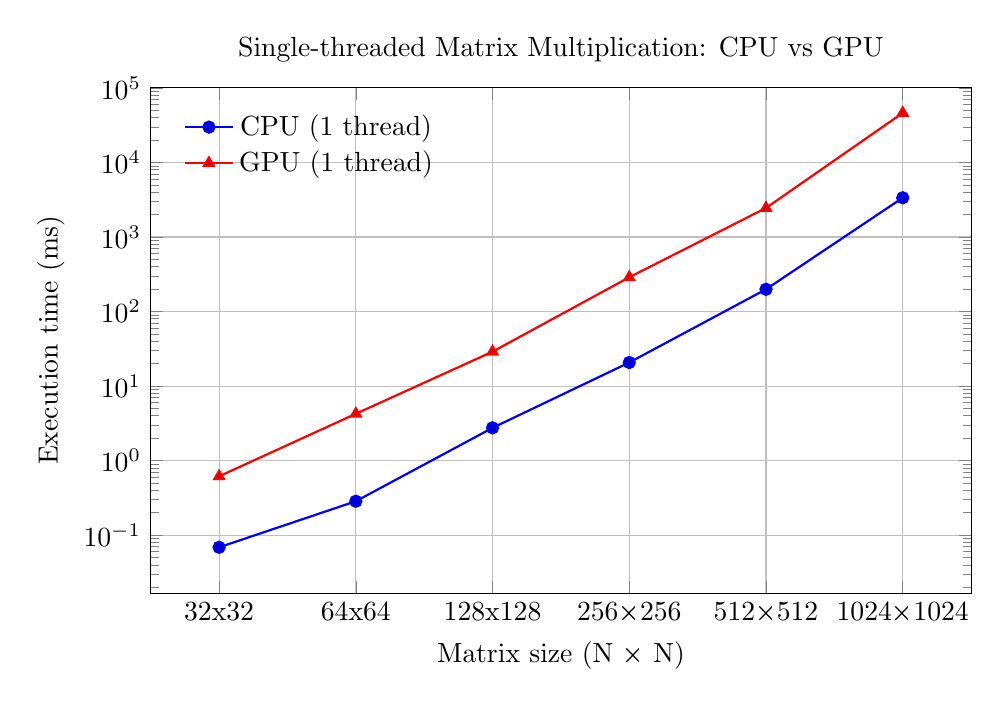
\begin{tikzpicture}
\begin{axis}[
    ymode=log,
    log basis y=10,
    width=12cm,
    height=8cm,
    xlabel={Matrix size (N × N)},
    ylabel={Execution time (ms)},
    title={Single-threaded Matrix Multiplication: CPU vs GPU},
    legend pos=north west,
    xtick=data,
    xticklabels={32x32, 64x64, 128x128, 256×256, 512×512, 1024×1024},
    ymin=0,
    ymax=100000,
    grid=major,
    legend style={draw=none, fill=none}
]

\addplot+[mark=*, thick, blue] coordinates {
    (1, 0.068705)
    (2, 0.285104)
    (3, 2.751817)
    (4, 20.706290)
    (5, 198.716200)
	(6, 3356.762000)
};
\addlegendentry{CPU (1 thread)}

\addplot+[mark=triangle*, thick, red] coordinates {
    (1, 0.615584)
    (2, 4.249685)
    (3, 28.923530)
    (4, 287.943700)
    (5, 2446.466000)
    (6, 46097.410000)
};
\addlegendentry{GPU (1 thread)}

\end{axis}
\end{tikzpicture}

  }
  \caption{Single threaded Matrix Multiplication Execution between CPUs and GPUs averaged over 10 executions}
  \label{fig:singlethreadedgraph}
\end{figure}

\begin{figure}[H]
	\centering
	\resizebox{1.0\linewidth}{!}{
		\begin{tabular}{|r|r|r|r|r|}
\hline
\textbf{Matrix Size (n $\times$ n)} & \textbf{CPU Time (ms)} & \textbf{GPU Time (ms)} & \textbf{Speedup (GPU/CPU)} \\
\hline
32 $\times$ 32     & 0.068705   & 0.615584    & 11.970438 \\
64 $\times$ 64     & 0.285104   & 4.249685    & 15.554119 \\
128 $\times$ 128   & 2.751817   & 28.923530   & 11.419879 \\
256 $\times$ 256   & 20.706290  & 287.933700  & 13.906730 \\
512 $\times$ 512   & 198.716200 & 2446.466000 & 12.323010 \\
1024 $\times$ 1024 & 3356.762000 & 46097.410000 & 13.745850 \\
\hline
\end{tabular}


	}
	\caption{Data Matrix from Figure~\ref{fig:singlethreadedgraph}}
	\label{fig:singlethreadedmatrix}
\end{figure}	


As seen in Figure~\ref{fig:singlethreadedgraph} and Figure~\ref{fig:singlethreadedmatrix}, GPUs struggle in applications that fail to utilize the architectural parallelism. 
For each of the matrices tested, the CPU is on average around 13 times faster than the \acs{GPU}. 
The \acs{GPU} should only be used in place of the \acs{CPU}, when the application is parallelizable and lacks complex control flow logic, otherwise the application is significantly delayed.

For the context of this thesis, any scheduler running on the GPU employing complex control logic will incur significant latency overhead.  
In general, scheduling decision, task management, and resource assignment, must follow a sequential control flow, as these processes lack inherent parallelism. 
Consequently, efficient GPU task management often relies on a CPU side scheduler to handle task queuing and resource allocation, with the GPU side component primarily focused on dispatching tasks to available compute units. 


\subsection{GPU Architecture}

The NVIDIA Tesla V100 GPU, based on the Volta architecture, was selected for this project due to its availability and suitability for high performance computing workloads.  
At a high level, the GPU features 5,120 CUDA cores, 640 Tensor Cores, delivering up to 7 TFLOPS of double precision performance. %https://images.nvidia.com/content/technologies/volta/pdf/tesla-volta-v100-datasheet-letter-fnl-web.pdf
The system has 16 GB of \acs{VRAM} and provides 900GB/s of bandwidth between on-chip memory and device memory.
The GPU interfaces with the host system over PCIe, allowing a theoretical maximum of 16GB/s for transfers between CPU memory and VRAM. 

The performance of \acs{GPU} is often limited by the disparity between compute throughput and memory transfer rates. 
While the GPU can execute arithmetic operations at extremely high speed, fetching and storing data from VRAM is comparatively slower, which can stall execution if memory accesses is not optimized.
Even slower are the memory transfers between host and \acs{VRAM} and must be minimized to avoid further bottlenecks or stalls. 
Understanding this imbalance is fundamental to design of efficient scheduling and memory access patterns, which are essential to fully exploit the device capabilities.
The following analysis of the V100's hardware architecture, will provide both the reasoning and implementation fundamentals for designing an efficient GPU scheduling strategy.  


\subsubsection{Thread Hierarchy and Execution Model}

From the programmer's perspective when assigning tasks, the GPU appears as an array of independent, highly parallelized processors, called \acsp{SM}.
Each \acs{SM} receives work in the form of \acsp{CTA}, blocks of threads executing the same instruction code, which define the organization and grouping of threads for execution. 
The executing \acs{CTA} is subdivided into warps, the smallest execution unit on the GPU, each consisting of 32 GPU threads executing instructions in lockstep. 
The lockstep execution ensures all threads within a warp execute the same instruction simultaneously. 
By enforcing lockstep execution, the GPU can schedule and dispatch threads to compute units with a simplified design allowing further parallelism. 

While lockstep execution enables efficient SIMD style throughput, it also introduces a potential performance hazard.
If threads within a warp follow different control flow paths, these threads diverge, and the GPU is forced to execute these different threads sequentially with respect to one another.
This serialization stalls part of the warp using masks, which disable the write back of the compute units.
In effect, thread divergence, reduces the effective parallelism and degrades performance. 

\subsubsection{SM Architecture}

The Tesla V100 GPU \acs{SM} architecture, contains 4 processing partitions, each with its own complete execution pipeline.
These partitions share an L1 instruction cache as well as a combined L1 data and shared memory cache, enabling threads within different warps of the same \acs{CTA} to efficiently access shared instructions and data. 
Within the each processing partition there is an L0 instruction cache, a warp scheduler, a dispatch unit, and multiple execution units.
An in depth view of each processing partition's architecture is provided in Figure~\ref{fig:processing_partition}, taken from the NVIDIA Volta Whitepages.

\begin{figure}[H]
  \centering
  \includegraphics[width=0.5\textwidth]{figures/output-006.png}
  \caption{SM Processing Partition Architecture taken from the Volta Whitepages} %https://images.nvidia.com/content/volta-architecture/pdf/volta-architecture-whitepaper.pdf
  \label{fig:processing_partition}
\end{figure}

Every clock cycle, the warp scheduler selects a warp of 32 threads to issue to the dispatch unit, which dispatches decoded instructions to the appropiate functional units. 
If there are not enough execution units of the required type for a given instruction, the instruction is queued. 
Depending on the current queue and delays, such as global memory accesses or dependencies, the warp scheduler will interweave different instructions from other ready warps, ensuring that the execution units remain busy.
This thread interweaving allows GPUs to hide latencies and resource contention through thread oversubscription.
Beyond, the warp scheduler and dispatcher, each processing partition contains a number of execution units. 
In particular, there are Tensor Cores for deep learning, 64 bit-\ac{FP} cores, \ac{LD/ST} units, a register file, and \acs{SFU}s for mathematical functions such as sine and square root. 

\subsubsection{SM Scaling and Thread Concurrency}
Compared to CPU hardware threads, GPUs scale far more aggressively, supporting a much larger number of threads. 
On the Tesla V100, there are 80 individual \acsp{SM}, each capable of supporting up to 64 resident warps.
With 32 threads per warp, this yields $64 \times 32 = 2048$ threads per \acs{SM}. 
Across all 80 \acsp{SM}, the theoretical maximum concurrency is $80 \times 2048 = 163{,}840$ resident threads.
For comparison, a typical Intel Tiger Lake i5-1135G7 CPU has 4 cores with 2 hardware threads each, for a maximum of 8 concurrent hardware threads, while high end server CPUs, such as the Intel Xeon Gold 6148, only support 20 hardware threads.  
Although the \acs{GPU} oversubscribes the number of warps and threads to hide latencies, the total number of dispatch and scheduling units allow for a maximum of $4 * 32 * 80 = 10840$ instructions issued per cycle when the hardware is fully utilized. 


In practice, this theoretical maximum is rarely achieved due to resource bottlenecks.
All threads within an \acs{SM} share the same on-chip L1 data and shared memory cache, as well as the 256\,KiB on-chip register file ($16{,}384 \times 32$\, bit registers per processing partition, with four partitions per \acs{SM}).
\acs{SM} threads all share the same on-chip L1 data and shared memory cache and the 256KiB on-chip register file ($16{,}384 \times 32$\, bit registers per processing partition, with four partitions per \acs{SM}).
Depending on the kernel's resource usage, high register pressure will cause the kernel launch will fail. 
Furthermore, if multiple thread blocks with high shared memory demands get scheduled to the same \acs{SM}, they will saturate the L1 data and shared memory cache and force frequent evictions and write backs to global memory.  
These hardware limits must be carefully considered when mapping tasks to \acsp{SM}.

The built-in hardware scheduler normally either handles these constraints or fails the kernel launch. 
Implementing a custom scheduler on top of the hardware scheduler, requires consideration of these GPU limitations. 
Forcing new scheduling behavior may conflict with or be constrained by the hardware scheduler’s own mechanisms.


\subsubsection{Scheduling and Task Mapping}

The specific mapping of tasks to \acs{SM}, \acs{TPC}, and \acs{GPC} is determined natively by the proprietary hardware scheduler, the GigaThread Engine. 
While the exact documentation is not public, this module maps \acsp{CTA} to the individual \acsp{SM} based a multitude of factors: hardware resources, parallelism, priorities, and dependencies.
Similarly, the global memory and L2 cache utilization are determined by the hardware and transparent to the programmer.
After the \acs{CTA} gets mapped to the specific \acs{SM}, the device code then executes till completion without interruption. 

The \acsp{CTA} is entirely managed by the \acs{SM} on which it is currently executing. 
As shown previously the \acs{SM} has its own execution pipelines, register files, shared memory and scheduling units on which the \acs{CTA} executes.
For \acsp{SM} to communicate with one another, they must use either the global on-chip device \acs{HBM2} or through the global L2 cache which is shared and coherent across all \acsp{SM}.
Although these memory accesses allows individual \acsp{SM} to communicate with each other, accesses require hundreds of cycles, which introduce further latencies when compared to local \acs{SM} L1 memory caches.
Ideally, the \acsp{SM} execute independently of one another and accumulate answers in global memory, skipping the high memory latency accesses of coordinating synchronous work.

\section{GPU Programming using the CUDA API}

NVIDIA \acsp{GPU} are intended to be used as computational accelerators for a host system, which manages and schedules tasks using CUDA. 
In this model, the \acs{GPU} acts as a standalone processor with its own independent memory and execution pipelines. 
For tasks to be scheduled on the GPU, the host process must first launch the process using the CUDA API. 
The CUDA API is an extension of  C++, which allows the CPU to interact with the GPU. 
Using CUDA, the host invokes device functions, called kernels, by specifying the number of threads and the memory parameters. 
These kernel calls are asynchronous, meaning that once the host issues the command, the GPU executes it independently, while the CPU can continue with other work or synchronize later as needed. 


\subsection{Kernel Launches}

The task of launching and running device code begins from a kernel launch, which passes the function, its parameters, pointers, and the grid and block dimensions to the \acs{GPU}.
The launch configuration specifies the number of \acsp{CTA} and their logical organization into dimensions.
Every block is then mapped to a single \acs{SM} and is constrained by that \acs{SM}’s hardware resources, including the maximum number of threads, registers, resident warps, and available shared memory. 
If no available \acs{SM} can meet these requirements, the kernel launch will fail.
Conversely, if a \acs{CTA} does not fully saturate the hardware resources of an \acs{SM}, additional further blocks may be scheduled concurrently on the same \acs{SM}.  

\subsection{Memory and Bandwidth Considerations}


Both the GPU and CPU maintain distinct memory regions for different hardware architectural and performance reasons.  
CPU memory is optimized for low latency access to support serial and branch heavy workloads, while GPU memory is optimized for extremely high bandwidth to sustain thousands of parallel threads, accepting higher latency in exchange.
These memories are connected by an interconnect such as PCIe or NVLink, whose bandwidth is far lower than that of the GPU’s local memory, making constant access to host memory impractical without significant performance loss.
By keeping data local, each processor can operate at full efficiency, and the GPU can execute kernels independently without frequent synchronization with the CPU.
This separation is thus a deliberate design choice to match each processor’s optimization goals, avoid bottlenecks from the limited interconnect speed, and enable independent execution.


As the memory regions are distinct, for the GPU to support the CPU with tasks, the CPU needs to use CUDA to allocate and send data to the GPU memory.
When transferring data from the host, the CUDA API does not have access to the \acs{CPU}'s disk memory and requires the memory to be pinned to the \acs{CPU}'s \acs{RAM}.
While the CUDA runtime can perform this pinning automatically, host arrays allocated directly in pinned memory using \lstinline[language=cuda]'cudaMallocHost()' or \lstinline[language=cuda]`cudaHostAlloc()` skip the added step of pinning memory and enable faster transfers. 
Particularity in applications that are bandwidth bottlenecked, this added transfer latency is significant.
If the pinned memory is too large; however, it restricts the memory availability for the programs currently running on the \acs{CPU}, which may degrade performance by forcing the swapping of memory to disk storage. 

In CUDA, understanding how memory is transferred and managed across the host and the device is crucial for optimizing performance.  
For the programmer, the device memory is partitioned into main memory, the \acs{VRAM}, with a size of 16 GB on the Tesla V100 architecture, as well as on chip memory. 
The programmer can decide between three different models of memory management \lstinline[language=cuda]`__constant__`, \lstinline[language=cuda]`__device__`, and \lstinline[language=cuda]`__shared__` memory.
Both constant and device memory are allocated to the global memory, with constant memory only being writeable by the \acs{CPU} and allowing faster access times due to the reduced coherency required.
The shared memory is shared among all warps and threads of a given \acs{SM} in the L1 data and shared memory cache.  
This memory is far more performant than device memory, but limited in size, due to its location on chip.


\subsection{Memory Coalescing}

For the GPU to coalesce memory operations and enable SIMD-style execution across multiple data points, each thread maintains registers that store its execution context, including its position in the grid. 
In PTX, these special registers provide unique identifiers such as threadIdx and blockIdx, which indicate a thread’s coordinates within its block and a block’s coordinates within the grid.
These identifiers are essential for structuring parallel computations and optimizing memory access patterns.
For example, when threads within a warp access consecutive memory locations, the hardware can coalesce those accesses into a single memory transaction, significantly improving throughput.


\subsection{Example Kernel Launch}


Consider the following example program, which allocates device memory and launches a kernel consisting of one block and 32 threads. 

\begin{lstlisting}[language=cuda,caption={Simple CUDA Kernel}, label={lst:simple-kernel}]
__global__ void increment(float *x) {
    x[threadIdx.x] += 1.0f;
}

int main() {
    const int N = 1024;
    float h_x[N];
    for (int i = 0; i < N; ++i)
        h_x[i] = i * 1.0f;

    float *d_x;
    cudaMalloc((void**)&d_x, N * sizeof(float));
    cudaMemcpy(d_x, h_x, N * sizeof(float), cudaMemcpyHostToDevice);

    increment<<<1, 32>>>(d_x);

    cudaMemcpy(h_x, d_x, N * sizeof(float), cudaMemcpyDeviceToHost);
    cudaFree(d_x);
    return 0;
}
\end{lstlisting}

The code block above depicts the launching and execution of a simple GPU kernel that demonstrates the memory allocation scheme used for executing kernel code.
The kernel itself is the execution of the \acs{GPU} device program denoted by \lstinline[language=cuda]`__global__` function, while the \lstinline`<<<_, _>>>` syntax enables the programmer to specifically partition their execution tasks across waiting threads. 
The first value in the \lstinline`<<<1,32>>>` determines the block dimensions, which are either given as an array or a 3 dimensional tensor. 
Similarily, the second value determines the thread dimensions in the same format as the block dimension. 
In particular, this code allocates a singular block with an array of 32 threads, which completely saturates a singular warp. 
These dimensional vectors allow the different threads to maintain lockstep execution, while processing different values of the same array, as seen by using the dimensional properties assigned to the individual threads by the runtime system. 

The main function, executed by the \acs{CPU} or host, initializes the parameters, executes the kernel and then copies the memory back. 
The host array, \lstinline[language=C++]`h_x` is allocated to the stack, which exists only in \acs{CPU} memory, which needs to be passed to the \acs{GPU}.
Passing the array by value, something common in C++ code, seems at first the most simple; however, poses two seperate issues.
Firstly, when passing arrays as parameters, they decay to pointers, which CUDA forbids, as the pointer passed to the device does not have any meaning.
Secondly, if the array were wrapped in a struct and passed to the function to circumvent the first issue, the array would be allocated to every single thread independently. 
In the example above, the array would be allocated 32 times, each independent from one another, taking up further memory bandwidth and both on chip and global device memory. 
In this case, each individual thread, would get the array passed by value, leading to a total 32 threads * 1024 floats * 4 bytes per float or 128KiB. 
Instead, them memory is allocated in the device memory, transferred once and each thread recieves only the device pointer \lstinline[language=C++]`d_x`, which can be used to copy the results back to the host.  





\subsection{CUDA Streams}

CUDA API calls are queued to the \acs{GPU} using cuda streams, which enforce the execution order of tasks.
\lstinline[language=cuda]{cudaStream_t} defines a command queue for the GPU, which is similar to a Linux file pointer in that it returns an index referring to the specific allocated stream.
Each stream allows the queuing of operations such as kernel launches, memory copies, and memory set operations.
Commands submitted to the same stream are executed sequentially in the order they were issued, ensuring deterministic behavior within that stream.
Multiple streams, however, can run concurrently, enabling overlapping execution of kernels and memory operations to maximize GPU utilization and improve overall performance.
By carefully managing streams, developers can optimize task parallelism and resource usage on the GPU.

The Tesla V100 GPU has two seperate hardware copy engines for copying data from the host to the device and back. 
The copy engines support the transfer in both directions, with one engine specifically being allocated for the unidirectional \acs{D2H} transfer and the other for \acs{H2D}.
Using only one stream for multiple kernels fails to maximize the device memory bandwidth. 
For example, consider the launch of two independent kernels, kernel A and kernel B, each on the same CUDA stream. 
Both A and B, allocate and copy memory onto the device, schedule their kernels and then copy the results back. 
Regardless of the ordering of API calls, both kernels can not run simultaneously or use both \acs{H2D} and \acs{D2H} copy engines simultaneously.

To best utilize the hardware and ensure correct results, a different stream need to be used for each synchronous kernel launch.  
Each kernel must remain in the same stream as the memory copys related to that stream in order to ensure the arguments used by the kernel are accurate and that the results are not prematurely returned. 
By placing each kernel in its own stream, the CUDA API, depending on the time and specific situation run multiple kernels, run kernels and memory transfers, or perform both \acs{D2H} and \acs{H2D} API calls simultaneously.

\section{GPU Programming Models for Real Time Systems}\label{chapter:Coroutines}

In order to meet urgent deadlines, systems need to prioritize and ensure the timely execution of critical tasks.
Prioritizing execution requires that high priority tasks are scheduled first when resources are available, and that their deadlines are still met even when resources are fully occupied. 
Achieving this responsiveness, requires preemption or context switching between resident tasks and scheduled critical tasks. 
In Apollo, this responsiveness is implemented through coroutines, which cooperatively yield execution to enable timely task switching.
Coroutines are particularly well suited to GPU scheduling, since GPUs lack integrated hardware preemption and therefore depend on cooperative mechanisms to maintain responsiveness.


\subsection{Coroutines}

Coroutines are a form of asynchronous programming that enables cooperative multitasking between functions.
Unlike traditional thread or process switches, which can occur at any time and requires a larger context, coroutine switches happen only at programmer defined suspension points. 
This makes them particularly useful for enabling runtime kernel task switching on the GPU. 
Here, execution of a kernel can be suspended to allow another kernel to run, and then later resumed without blocking other work.

A coroutine suspends execution by capturing its current context, known as the continuation, which contains the execution state needed for later resumption \cite{Zheng2022LuisaRender}.
Once suspended, another task can execute without overwriting or disrupting the saved kernel state.
When the interim task completes, the coroutine can continue exactly where it left off by restoring its continuation.
This ability to strategically pause and resume execution makes coroutines well suited for real time workloads, where rapid switching between concurrent tasks can help meet hard deadlines without delay.


\subsubsection{CPU Coroutines in Apollo}

Coroutines on the CPU are implemented using the native x86 calling conventions and the program stack to dynamically save and restore continuations.
Under x86 convention, when a function is invoked, the CPU pushes the return address, the location after the next instruction after the call, onto the stack before jumping to the target function.
The called function accesses its local variables through the stack and registers, which are divided into two categories, volatile, caller saved and non volatile, callee saved.
Volatile registers may be freely modified by the callee, while callee saved registers must be preserved and restored before the function returns.

When excecution reaches a return instruction, the CPU pops the return address off the stack and continues execution from that point.
To implement coroutine behaviour, however, the function must be able to yield and later resume.  
This requires saving the callee saved registers, since thier preservation is guaranteed, as well as any additional state such as local variables or registers, that is necessary for continued execution.
These elements can be stored on the stack, enabling a coroutine to pause and later continue seamlessly. 

The Apollo project demonstrates this mechanism with CPU coroutines implemented directly on top of the x86 calling convention, as illustrated in the following example. 

\begin{lstlisting}[language=x86asm,caption={CPU Coroutine}, label={lst:coro}]
ctx_swap:
    pushq %rdi
    pushq %r12
    pushq %r13
    pushq %r14
    pushq %r15
    pushq %rbx
    pushq %rbp
    movq %rsp, (%rdi)

    movq (%rsi), %rsp
    popq %rbp
    popq %rbx
    popq %r15
    popq %r14
    popq %r13
    popq %r12
    popq %rdi
    ret
\end{lstlisting}

The CPU coroutine implementation uses the context switching function, ctx\_swap, which captures the current continuation and restores the state of another coroutine. 
This function accepts two parameters, \texttt{\%rdi} and \texttt{\%rsi}, which point to the memory locations used to store and retrieve coroutine continuations.
Execution happens in two stages.
In the first stage, the continuation is stored and its address is saved to the register \texttt{\%rdi}.  
The second stage then moves the stack frame to the location of its continuation, using the register \texttt{\%rsi}, before restoring the new coroutine context.

Each stage loads or saves their registers in a specific defined order. 
In particular, to ensure the memory is reread into the correct registers, the order of pushing elements onto the stack is the reverse order of popping elements. 
As the stack works on a last in first out principle, this ensures that all the registers have the correct values upon resumption. 
In comparison to traditional context switches involving processes or threads, coroutine context switching via ctx\_swap operates with significantly lower overhead, resulting in faster execution.

\subsection{GPU Coroutines}

Unlike CPU coroutines, which can implement context switching by saving and restoring stack frames, GPUs cannot use the same mechanism, as GPU threads do not maintain conventional stack frames.
Instread, their execution state is managed differently, requiring specialized approaches to preserve and resume coroutine execution.

Attempting to implement CPU style coroutines using the ctx\_swap function does not work because GPUs handle function calls differently.
\acsp{CPU} stores a call stack of function stack frames, which can be easily accessed and manipulated by pushing and popping values or addresses.
\acsp{GPU}, in contrast, avoids traditional stack frames by aggressively inlining function calls, reducing overhead since function code is readily available and no stack frame is needed. 

Implementing and manipulating deep call stacks on GPUs is largely handled by the compiler and hardware, leaving very little control to the programmer, which makes such approaches impractical.
For example, CUDA originally did not support recursive functions, which were only introduced later via the \lstinline[language=cuda]`-rdc=true` flag. 
Even then, recursion comes with strict limitations on stack size and adds significant performance overhead.
Attempting to rely on deep call stacks can quickly lead to excessive instruction and register usage, illustrating why GPU architectures and compilers discourage CPU style stack manipulation.

\subsubsection{Persistent Threads to support Coroutines}

Given that call stacks are not effectively or efficiently supported in CUDA, the GPU needs to support a user level runtime scheduling mechanism to manage the contexts dynamically. 
Due to the nature of kernels executing until completion, the \acs{GPU} coroutine scheduler needs to be based on a persistent kernel, which can schedule coroutines throughout the lifetime of the application.
The coroutines running on the persistent threads will then define suspension points to manually give control back to the scheduler in order to switch tasks. 
Because storing every register for all threads across coroutines is too expensive and inaccessible, coroutine contexts must be explicitly synthesized and saved in global memory, freeing the limited \acs{SM} resources for new tasks.

\subsection{Persistent Kernels}

Persistent GPU threads give the programmer enhanced control over hardware scheduling by running on top of the hardware scheduler, enabling manual execution decisions that are otherwise unavailable.  
In addition to this increased flexibility, persistent kernels reduce runtime scheduling overhead.
As the hardware resources are preallocated, thread and block configurations are loaded ahead of execution, the runtime avoids repeatedly configuring these settings, allowing kernels to run more efficiently. 
In systems with recurring or periodic tasks, such as autonomous driving, this overhead becomes particularly costly. 
With the implementation of persistent threads, only input and output buffers need to be updated for each new task, minimizing execution overhead and allowing kernels to operate with only the essential arguments required for computation.





